\documentclass[eng,openany]{mgr}
\usepackage{listings}
\usepackage[english]{babel}
\usepackage{graphicx}
\usepackage{hyperref}
\usepackage{tabularx,colortbl} 
\usepackage{rotating}
\usepackage[utf8]{inputenc} 
\setlength\parindent{24pt}
\usepackage[parfill]{parskip}
\usepackage[table,kernelfbox,hyperref]{xcolor}
\usepackage{fancyhdr}
\usepackage{gauss}
%\usepackage[colorinlistoftodos]{todonotes}

\hypersetup{colorlinks=true}
\hypersetup{xurlbordercolor=red!70!black}
\hypersetup{xlinkbordercolor=blue!70!black}
\hypersetup{linkcolor=blue!60!black}
\hypersetup{urlcolor=red!50!black}
\hypersetup{citecolor=green!30!black}
\rfoot{Page \thepage}
\renewcommand\lstlistlistingname{List of Listings}
\newcommand{\linia}{\rule{\linewidth}{0.4mm}}

\definecolor{listlightgray}{gray}{0.93}

\newcommand{\lstsetmylst} {
\lstset{frame = tb,
breaklines=true,
framerule = 0.25pt,
float,
fontadjust,
backgroundcolor={\color{listlightgray}},
basicstyle = {\ttfamily\footnotesize},
identifierstyle = {\ttfamily},
stringstyle = {\ttfamily},
showstringspaces = false,
showtabs = false,
numbers = left,
numbersep = 6pt,
tabsize = 4,
language=C,
floatplacement=!h
}
}

\newcommand{\lstsetatc} {
\lstset{frame = tb,
breaklines=true,
framerule = 0.25pt,
float,
fontadjust,
backgroundcolor={\color{listlightgray}},
basicstyle = {\ttfamily\footnotesize},
keywordstyle = {\ttfamily\color{listkeyword}\textbf},
identifierstyle = {\ttfamily},
commentstyle = {\ttfamily\color{listcomment}\textit},
stringstyle = {\ttfamily},
showstringspaces = false,
showtabs = false,
numbers = left,
numbersep = 6pt,
numberstyle={\ttfamily\color{listnumbers}},
tabsize = 4,
language=C,
floatplacement=!h
}
}

\newcommand{\lstsetatbashnum} {
\lstset{frame = tb,
breaklines=true,
framerule = 0.25pt,
aboveskip=2ex,
float,
fontadjust,
backgroundcolor={\color{listlightgray}},
basicstyle = {\ttfamily\footnotesize},
keywordstyle = {\ttfamily\color{listkeyword}\textbf},
identifierstyle = {\ttfamily},
commentstyle = {\ttfamily\color{listcomment}\textit},
stringstyle = {\ttfamily},
showstringspaces = false,
showtabs = false,
numbers = left,
numbersep = 6pt,
numberstyle={\ttfamily\color{listnumbers}},
tabsize = 4,
language=bash,
floatplacement=!h
}
}
\lstsetmylst
\author{Jaroslaw M. Szumega}
\title{}
\engtitle{}
\supervisor{Rafal Zdunek, D.Sc, K-4/W4}
\field{Electronics}
\specialisation{Advanced Applied Electronics}
\date{02.06.2017}
\begin{document}
\selectlanguage{english}
\maketitle
\tableofcontents
\newpage

\chapter{Solution to the given problems}
\begin{figure}[h]
\centering
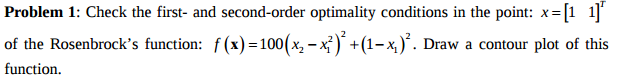
\includegraphics[width=0.7\linewidth]{screenshot001}
\label{fig:screenshot001}
\end{figure}

The first step will be expanding the given function, so further we can calculate the derivatives for gradient:\\
\begin{flalign*}
f(x) &= 100(x_2 - x_1^2)^2 + (1 - x_1)^2 \\
&= 100 (x_2^2 - 2x_2x_1^2 + x_1^4) + (1 - 2x_1 + x_1^2) \\
&= 100x_2^2 - 200x_2x_1^2 + 100x_1^4 + 1 - 2x_1 + x_1^2 \\
&= 100x_1^4 + x_1^2 - 2x_1 + 100x_2^2 - 200x_2x_1^2 + 1
\end{flalign*}
\\
\\
And the point to check is:\\
\begin{math}
x = [x_1\ x_2]^T = [1\ 1]^T
\end{math}

The First order optimality condition is:\\
\begin{flalign*}
\nabla f(x^*) &= 0\\ \\
\frac{\delta f(x)}{\delta x_2} &= 400x_1^3 + 2x_1 -2 - 400x_2x_1\\
&= 400 + 2 - 2 - 400 = 0\\ \\
\frac{\delta f(x)}{\delta x_1} &= 200x_2 - 200x_1^2\\
&= 200 - 200 =  0
\end{flalign*}

In given point x = [1 1] the first--order optimality condition is fulfilled.

The Second order optimality condition is:\\
\begin{flalign*}
\nabla f(x^*) &= 0\ (calculated\ in\ previous\ step)\\ \and
\nabla^2 f(x^*)\ &= positive\ semi-definite\ matrix\\ \\
\nabla^2 f(x^*)\ &= 
\begin{bmatrix}%
\frac{\delta^2 f(x)}{\delta x_1^2} & \frac{\delta^2 f(x)}{\delta x_1x_2}\\
\frac{\delta^2 f(x)}{\delta x_1x_2} & \frac{\delta^2 f(x)}{\delta x_2^2}
\end{bmatrix}\\
&=
\begin{bmatrix}%
1200x_1^2 + 2 - 400x_2& - 400x_1\\
-400x_1& 200
\end{bmatrix}\\
for\ point\ [1\ 1] &=
\begin{bmatrix}%
1200 + 2 - 400& - 400\\
-400& 200
\end{bmatrix}\\
H &=
\begin{bmatrix}%
802& -400\\
-400& 200
\end{bmatrix}
\end{flalign*}
As it can be noticed, all principal minors are positive ($H_{1,1}\ and\ H_{2,2}$). Therefore the $H(x_*)$ is positive semi-definite.\\
\\
Octave code below was written to plot contour for this task.
\begin{lstlisting}
pkg load symbolic

syms x1 x2
f = @(x1,x2) 100.*(x2 - x1.^2).^2 + (1 - x1).^2;

ezcontour(f,[-3,3])
\end{lstlisting}

\begin{figure}[h]
\centering
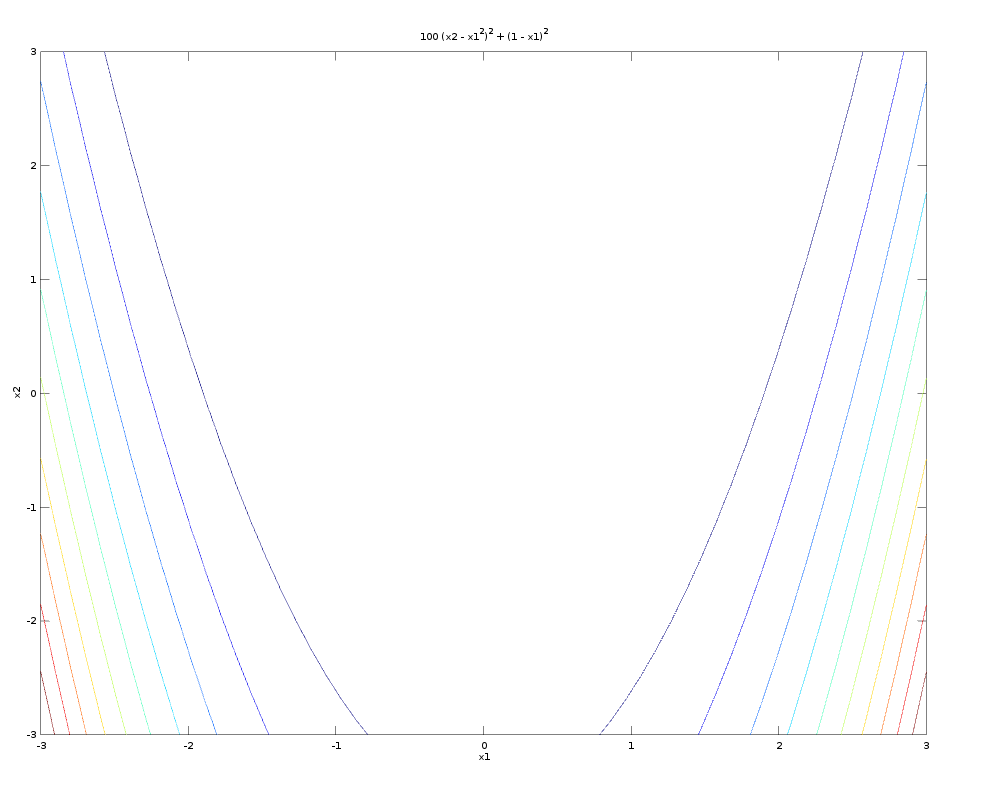
\includegraphics[width=0.7\linewidth]{screenshot002}
\caption{Contour plot of given function.}
\label{fig:screenshot002}
\end{figure}
\newpage
\begin{figure}[h]
	\centering
	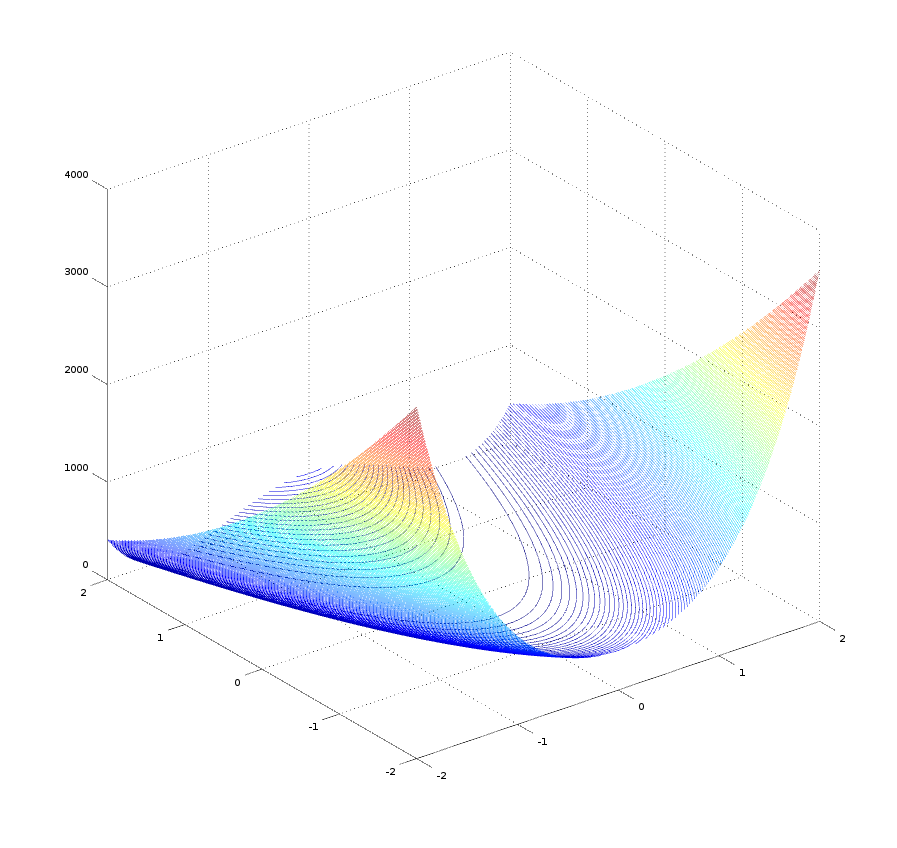
\includegraphics[width=0.7\linewidth]{screenshot007}
	\caption{Contour plot of function in 3D version.}
	\label{fig:screenshot007}
\end{figure}

\newpage

\begin{figure}[h]
	\centering
	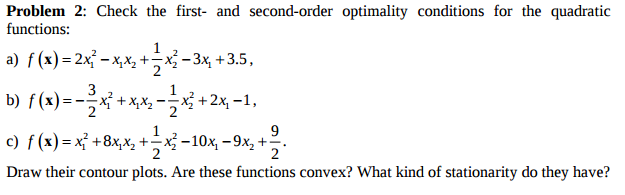
\includegraphics[width=0.7\linewidth]{screenshot003}
	\label{fig:screenshot003}
\end{figure}
Just like in the first task, we need to calculate the gradient and Hessian.//
Then it can be determined which type of stationarity the functions have.
\textbf{Point a)}
\\
\begin{align*}
f(x) &= 2 x_{1}^{2} - x_{1} x_{2} - 3 x_{1} + \frac{x_{2}^{2}}{2} + 3.5\\
\nabla f(x^*) &= 0\\ \\
\frac{\delta f(x)}{\delta x_2} &= 4 x_{1} - x_{2} - 3
\\
\frac{\delta f(x)}{\delta x_1} &= - x_{1} + x_{2}
\\
\end{align*}
To ensure the equality to zero, we can calculate that stationary point shall be:
\begin{align*}
x_1\ &=\ 1\\
x_2\ &=\ 1
\end{align*}

Now we will calculate the Hessian:
\begin{flalign*}
\nabla f(x^*) &= 0\ (calculated\ in\ previous\ step)\\ \and
\\
\nabla^2 f(x^*)\ &= 
\begin{bmatrix}%
\frac{\delta^2 f(x)}{\delta x_1^2} & \frac{\delta^2 f(x)}{\delta x_1x_2}\\
\frac{\delta^2 f(x)}{\delta x_1x_2} & \frac{\delta^2 f(x)}{\delta x_2^2}
\end{bmatrix}\\
&=
\begin{bmatrix}%
4& - 1\\
-1& 1
\end{bmatrix}\\
H &=
\begin{bmatrix}%
4& - 1\\
-1& 1
\end{bmatrix}\\
\end{flalign*}
To establish the type of stationarity we need to check Hessian determinant and the values of principal minors:
\begin{align*}
det(H)\ =\ 4\ +\ 1\ =\ 5\ >\ 0\\
H_{1,1}\ =\ 1\ >\ 0\\
H_{2,2}\ =\ 4\ >\ 0\\
\end{align*}

The Hessian is strictly positive definite, so we have the minimizer at calculated point.\\
\\

\begin{figure}[h]
	\centering
	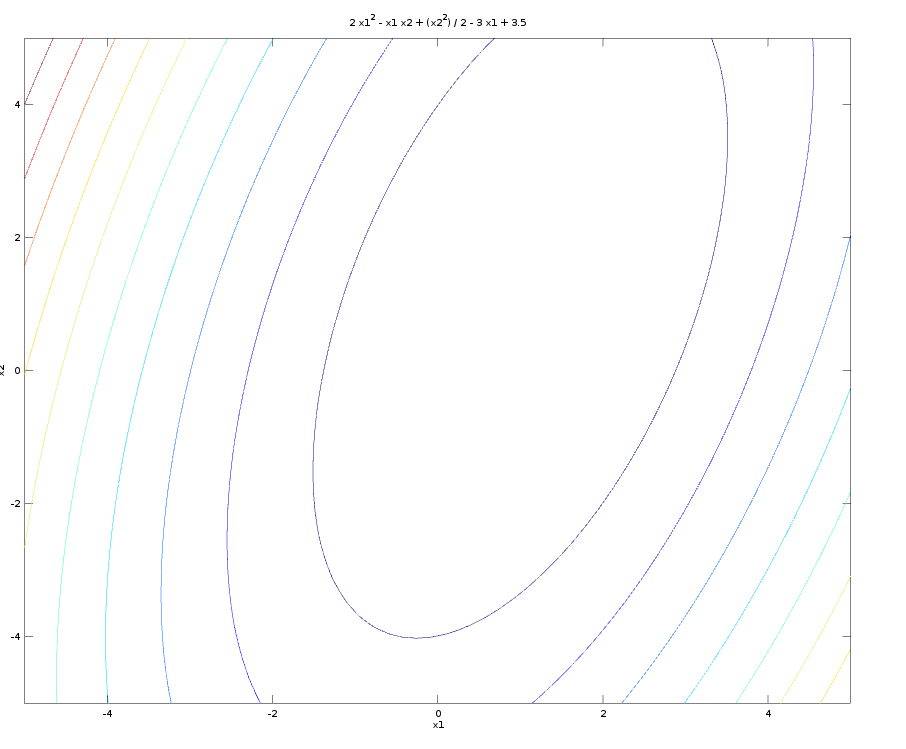
\includegraphics[width=0.7\linewidth]{screenshot004}
	\caption{Contour plot of point a) function.}
	\label{fig:screenshot004}
\end{figure}

\begin{figure}[h]
\centering
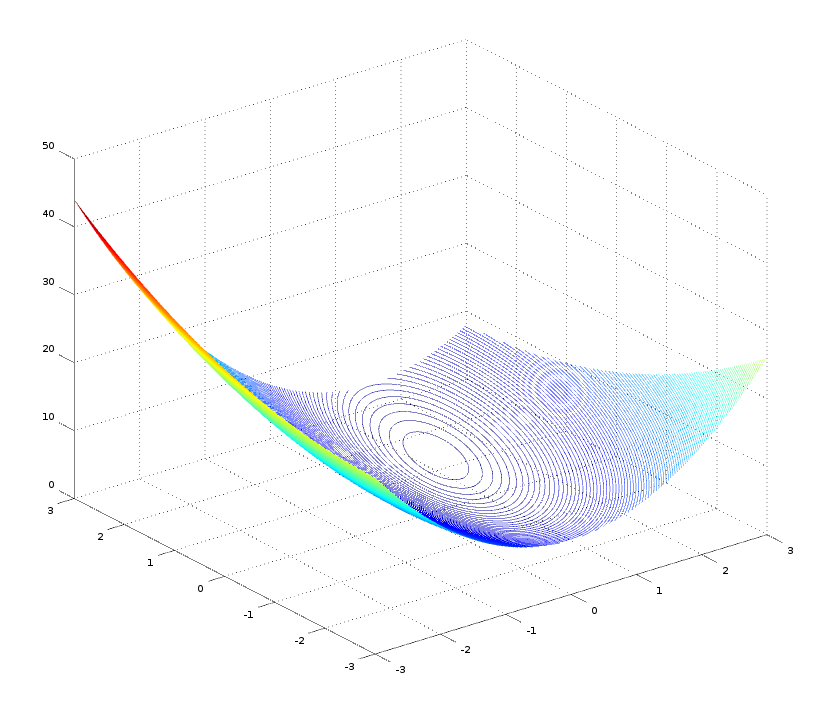
\includegraphics[width=0.7\linewidth]{screenshot008}
\caption{And its 3D version. We can notice the minimum.}
\label{fig:screenshot008}
\end{figure}

\clearpage

\textbf{Point b)}
\begin{align*}
f(x) &= - \frac{3 x_{1}^{2}}{2} + x_{1} x_{2} + 2 x_{1} - \frac{x_{2}^{2}}{2} - 1\\
\nabla f(x^*) &= 0\\ \\
\frac{\delta f(x)}{\delta x_2} &= - 3 x_{1} + x_{2} + 2
\\
\frac{\delta f(x)}{\delta x_1} &= x_{1} - x_{2}
\end{align*}
The calculated values for fulfilling the condition of $\nabla f(x^*) = 0$:
\begin{align*}
x_1\ &=\ 1\\
x_2\ &=\ 1
\end{align*}

Now we will calculate the Hessian:
\begin{flalign*}
\nabla f(x^*) &= 0\ (calculated\ in\ previous\ step)\\ \and
\\
\nabla^2 f(x^*)\ &= 
\begin{bmatrix}%
\frac{\delta^2 f(x)}{\delta x_1^2} & \frac{\delta^2 f(x)}{\delta x_1x_2}\\
\frac{\delta^2 f(x)}{\delta x_1x_2} & \frac{\delta^2 f(x)}{\delta x_2^2}
\end{bmatrix}\\
&=
\begin{bmatrix}%
-3& 1\\
1& -1
\end{bmatrix}\\
H &=
\begin{bmatrix}%
-3& 1\\
1& -1
\end{bmatrix}\\
\end{flalign*}
To establish the type of stationarity we need to check Hessian determinant and the values of principal minors:
\begin{align*}
det(H)\ =\ 3\ -\ 1\ =\ 2\ >\ 0\\
H_{1,1}\ =\ -1\ <\ 0\\
H_{2,2}\ =\ -3\ <\ 0\\
\end{align*}
The Hessian is strictly negative definite, The maximizer is present.
\\
\begin{figure}[h]
\centering
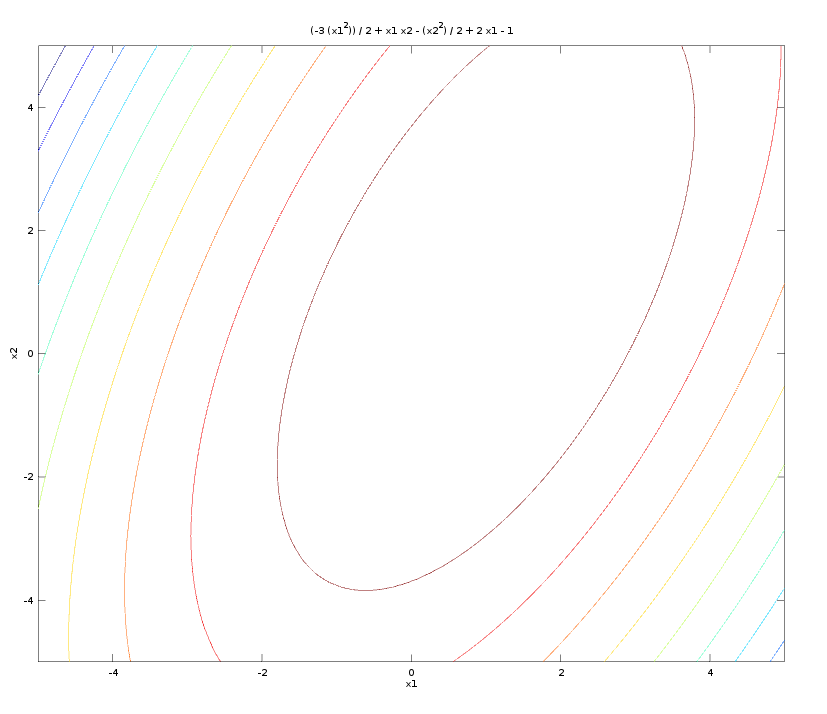
\includegraphics[width=0.7\linewidth]{screenshot005}
\caption{Contour plot of point b) function.}
\label{fig:screenshot005}
\end{figure}

\begin{figure}
\centering
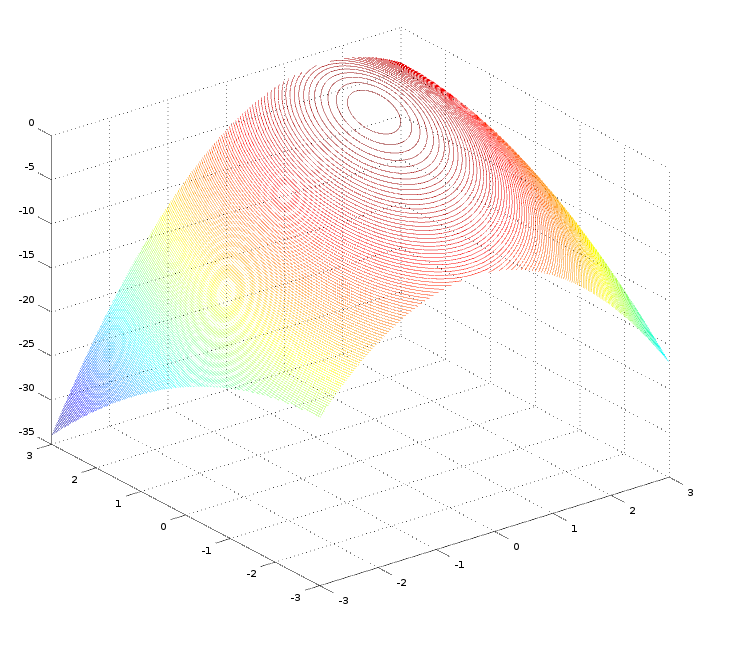
\includegraphics[width=0.7\linewidth]{screenshot009}
\caption{3D version with maximum observed.}
\label{fig:screenshot009}
\end{figure}


\clearpage
\textbf{Point c)}

In third point, the following function needs to be analyzed:
\begin{align*}
f(x) &= x_{1}^{2} + 8 x_{1} x_{2} - 10 x_{1} + \frac{x_{2}^{2}}{2} - 9 x_{2} + 4
\end{align*}

The task routine remains all the same as before:
\begin{align*}
\nabla f(x^*) &= 0\\ \\
\frac{\delta f(x)}{\delta x_2} &= 2 x_{1} + 8 x_{2} - 10
\\
\frac{\delta f(x)}{\delta x_1} &= 8 x_{1} + x_{2} - 9
\\
\end{align*}
To ensure the equality to zero, we can calculate that stationary point shall be:
\begin{align*}
x_1\ &=\ 1\\
x_2\ &=\ 1
\end{align*}

Now we will calculate the Hessian:
\begin{flalign*}
\nabla f(x^*) &= 0\ (calculated\ in\ previous\ step)\\ \and
\\
\nabla^2 f(x^*)\ &= 
\begin{bmatrix}%
\frac{\delta^2 f(x)}{\delta x_1^2} & \frac{\delta^2 f(x)}{\delta x_1x_2}\\
\frac{\delta^2 f(x)}{\delta x_1x_2} & \frac{\delta^2 f(x)}{\delta x_2^2}
\end{bmatrix}\\
&=
\begin{bmatrix}%
2& 8\\
8& 1
\end{bmatrix}\\
H &=
\begin{bmatrix}%
2& 8\\
8& 1
\end{bmatrix}\\
\end{flalign*}
To establish the type of stationarity we need to check Hessian determinant and the values of principal minors:
\begin{align*}
det(H)\ =\ 2\ -\ 64\ =\ -62\ <\ 0\\
\end{align*}
The determinant of Hessian is smaller than zero -- at this point we know that the critical point of function is a saddle point.
\\


\begin{figure}[h]
\centering
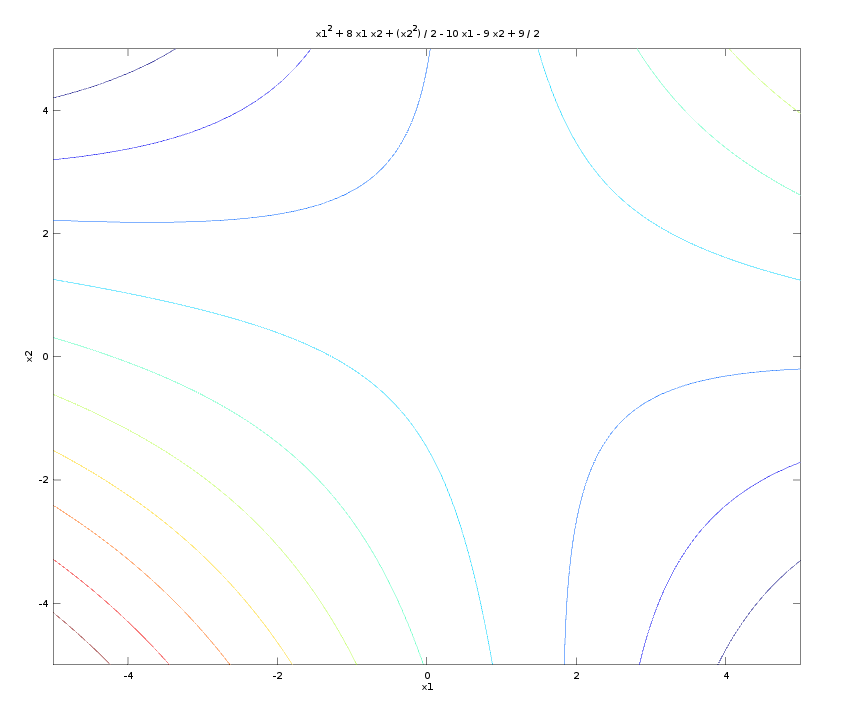
\includegraphics[width=0.7\linewidth]{screenshot006}
\caption{The contour plot of point c) function.}
\label{fig:screenshot006}
\end{figure}

\begin{figure}[h]
\centering
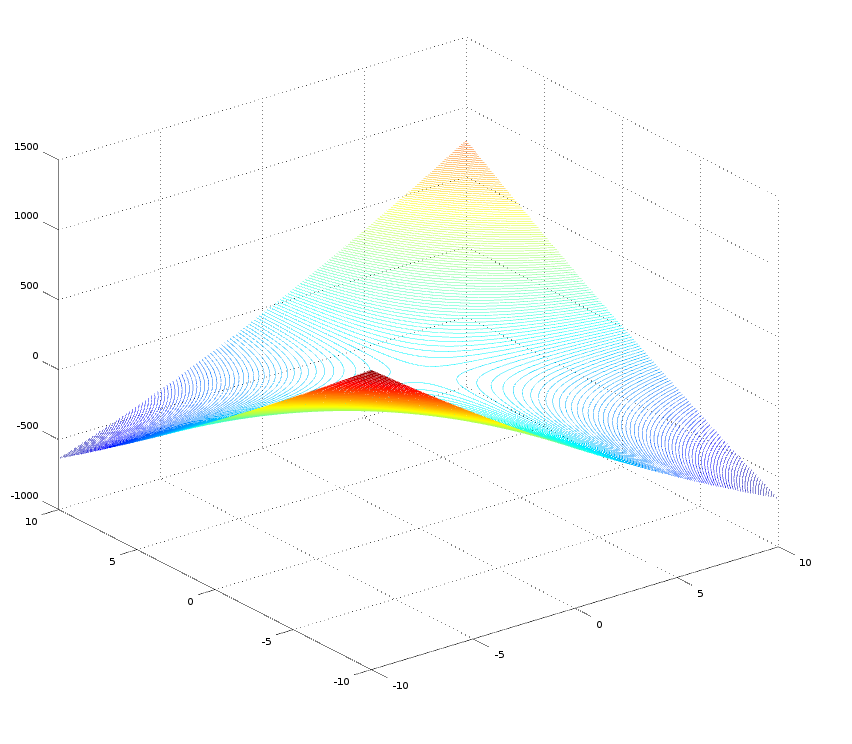
\includegraphics[width=0.7\linewidth]{screenshot010}
\caption{Visualization of point c) saddlepoint.}
\label{fig:screenshot010}
\end{figure}

\clearpage
\begin{figure}[h]
\centering
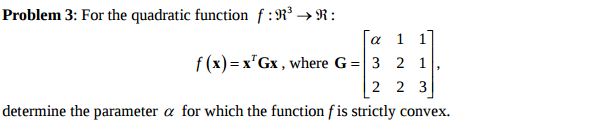
\includegraphics[width=0.7\linewidth]{screenshot011}
\label{fig:screenshot011}
\end{figure}

To ensure the function is convex, the Hessian matrix of the function
has to be strictly positive--definite.
\\
\\
\begin{math}
\nabla^2 f(x^*)\ = (x^TGx)'' = 2G\\
\\
H = 
\begin{bmatrix}
2\alpha & 2 & 2\\
6& 4& 2\\
4& 4& 6\\
\end{bmatrix}
\end{math}

Following the requirements, it needs to fulfill the following conditions:
\begin{itemize}
	\item matrix determinant $>$ 0,
	\item first principal minor $>$ 0.
\end{itemize}
So now we establish the determinant:\\
\begin{align*}
det(H) &= 48\alpha + 16 + 48 - 32 - 16\alpha - 72\\
 &= 32 \alpha - 40
 \\
 32\alpha -40 &> 0\\
 4\alpha -5 &> 0\\
 \alpha &> 5/4
\end{align*}

And the first principal minor:\\
\begin{align*}
det(M1) &= 8\alpha - 12\\
\\
8\alpha -12 &> 0\\
2\alpha -3 &> 0\\
\alpha &> 3/2
\end{align*}

In the end, if $alpha > 1.5$, then the given function will be convex.
\clearpage 

%task4
\begin{figure}[h]
\centering
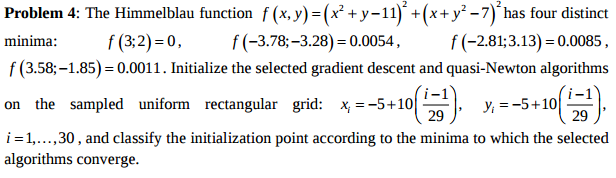
\includegraphics[width=0.7\linewidth]{screenshot012}
\label{fig:screenshot012}
\end{figure}

For better insight of the problem, the contour plot of the Himmelblau function was shown/
\begin{figure}[h]
\centering
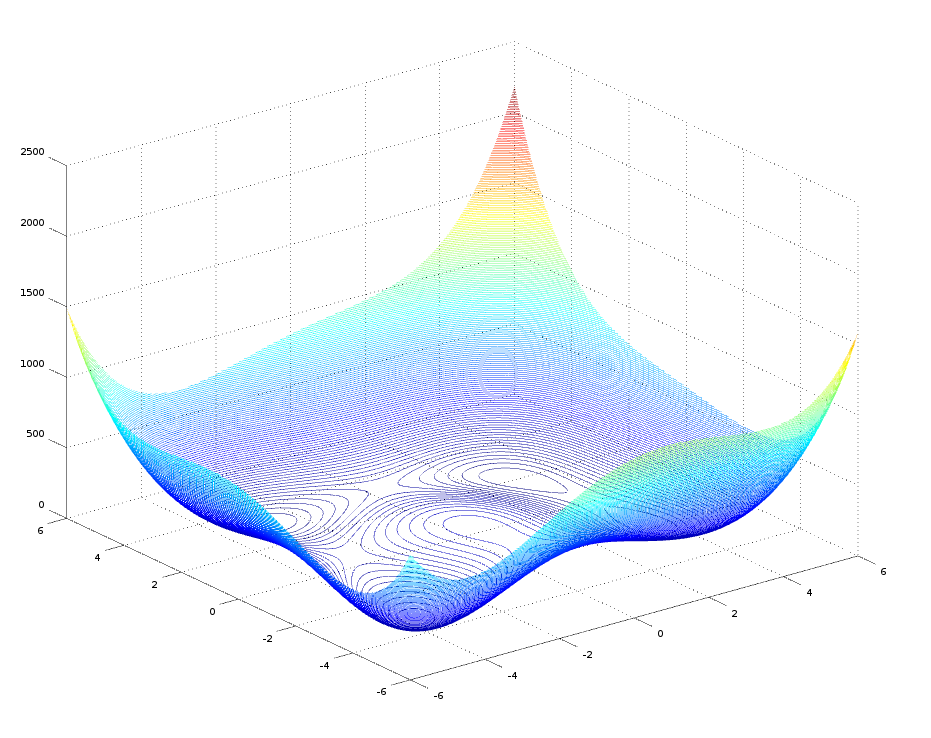
\includegraphics[width=0.7\linewidth]{screenshot013}
\caption{Contour plot of Himmelblau function.}
\label{fig:screenshot013}
\end{figure}

On the figure \ref{fig:screenshot013} can observe the four regions that are supposed to be the listed minimas.\\ \\
Considering the nature of the presented function, we can assume that depending on the starting point the algorithms will hit one of them. Of course there is also a possibility that method would not converge and will give a result that is not expected.
\\
\\
At the very beginning, there was an variant of the coded functions that symbolically calculated the necessary functions:
\begin{lstlisting}
function [f0,g0] = himmelblau(xp)

syms x y
f = (x.^2 + y - 11).^2 + (x + y.^2 - 7).^2;
fs = function_handle(f);
f0 = fs(xp(1),xp(2));

g = gradient(f)';
gs = function_handle(g);
g0 = gs(xp(1),xp(2));

endfunction
\end{lstlisting}
Unfortunately, it turned out, that it is not the best approach. The calculations time was long -- it took almost 70 seconds to calculate the minimum for one entry:
\begin{lstlisting}
Entry = [5, 5]

solution = 
-3.7793  -3.2832
Elapsed time is 66.5192 seconds.
\end{lstlisting}
Definitely, it is too long. So it was decided to hardcode the function and its gradient in a form that can be directly evaluated with argument in the future:
\begin{lstlisting}
function [f,gf] = himmelblau_explicit(x)
	f = (x(1).^2 + x(2) - 11).^2 + (x(1) + x(2).^2 - 7).^2;
	
	gf = [2*(2*x(1)*(x(1).^2 + x(2) - 11) + x(1) + x(2).^2 - 7); 2*(x(1).^2 + 2*x(2)*(x(1) + x(2).^2 - 7) + x(2) - 11)];
end
\end{lstlisting}

The explicit way of defining either function and gradient resulted in great speed--up (it is over 300x faster than symbolic operations). \begin{lstlisting}
Entry = [5, 5]

solution =
-3.2832  -3.2832
Elapsed time is 0.021183 seconds.
\end{lstlisting}


The table on the \ref{fig:screenshot014} presents the result of used algorithms.
\begin{figure}[h]
\centering
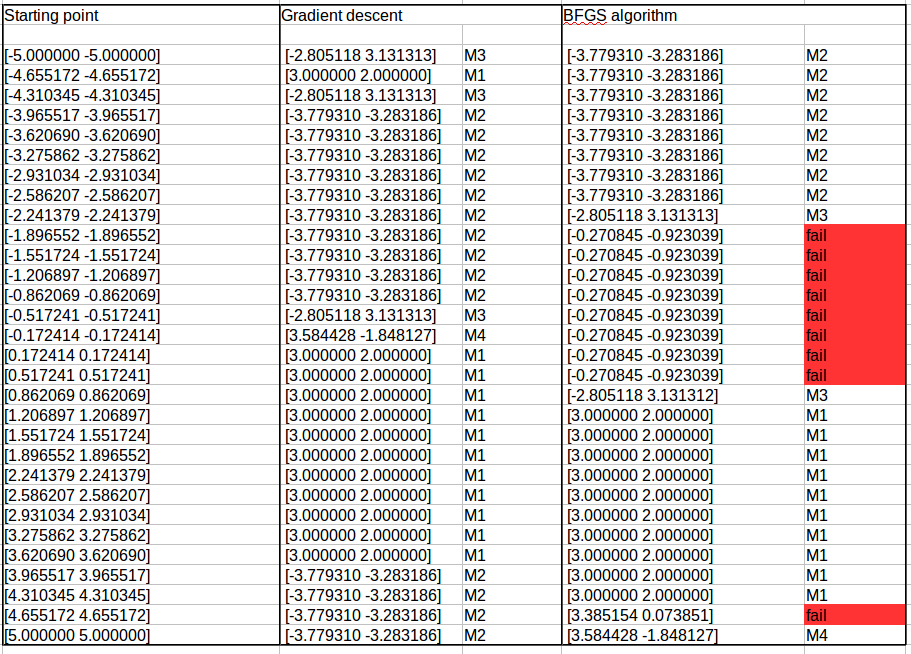
\includegraphics[width=0.8\linewidth]{screenshot014}
\caption{Starting point along with the corresponding hit minima for each algorithms.}
\label{fig:screenshot014}
\end{figure}

\clearpage

\begin{figure}[h]
\centering
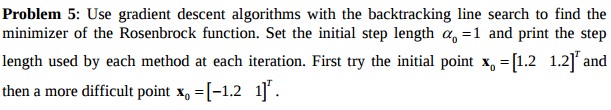
\includegraphics[width=0.7\linewidth]{screenshot015}
\label{fig:screenshot015}
\end{figure}


\begin{figure}[h]
\centering
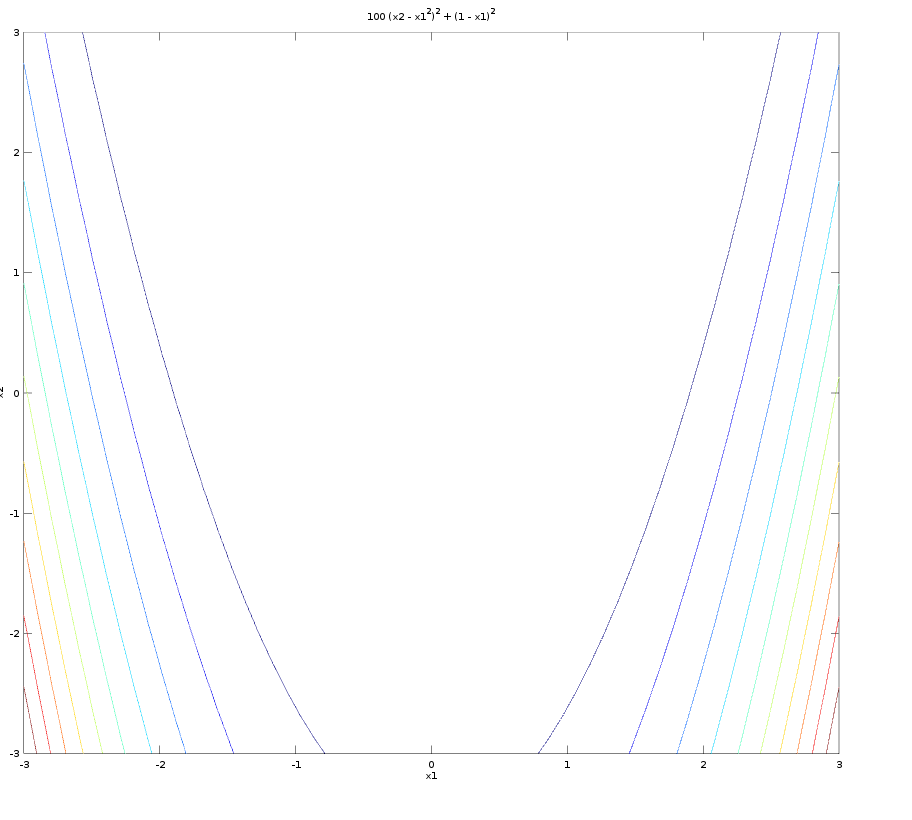
\includegraphics[width=0.5\linewidth]{screenshot019}
\label{fig:screenshot019}
\end{figure}

\begin{figure}[h]
\centering
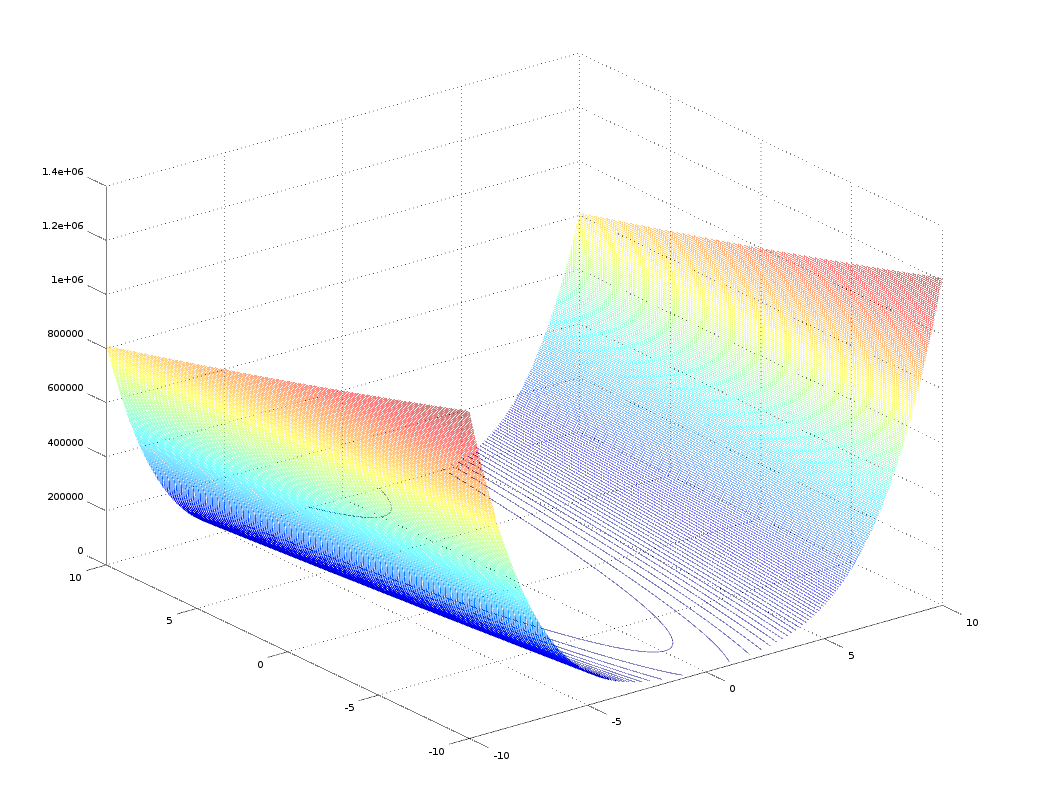
\includegraphics[width=0.5\linewidth]{screenshot018}
\caption{Two contour plots of the Rosenbrock functions (called also the valley/banana function.)}
\label{fig:screenshot018}
\end{figure}
There was trial of calculus using both initial points. Gradient Descent in the first case found the minimum [1, 1]:
\begin{lstlisting}
x1 = [1.2, 1.2]

iterations  =  13013

solution =
1.0000   1.0000

Elapsed time is 22.0776 seconds.
\end{lstlisting} 
In the case of "more dificult" initial point, the GS algorithm was stuck. Running in debug mode has proven that it fail during backtracking search and goes into infinite loop.

Here is also requested print of step lengths (shortened a little because of amount of steps taken):
\begin{lstlisting}
iteration =  100
a =    9.7656e-04
iteration =  200
a =    9.7656e-04
iteration =  300
a =    9.7656e-04
iteration =  400
a =    9.7656e-04
iteration =  500
a =    9.7656e-04
iteration =  600
a =  0.015625
iteration =  700
a =  0.0019531
iteration =  800
a =  0.0019531
iteration =  900
a =  0.0019531
iteration =  1000
a =  0.0019531

iteration =  2000
a =  0.0019531

iteration =  7000
a =  0.0019531

iteration =  9000


iteration =  10300
a =  0.0019531
iteration =  10400
a =  0.0039062

a =  0.0019531
iteration =  13000
a =  0.0019531
\end{lstlisting}






















\clearpage
\begin{figure}[h]
\centering
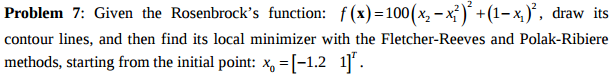
\includegraphics[width=0.7\linewidth]{screenshot016}
\label{fig:screenshot016}
\end{figure}










\clearpage
\begin{figure}[h]
\centering
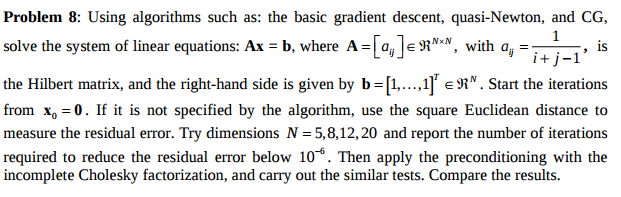
\includegraphics[width=0.7\linewidth]{screenshot017}
\label{fig:screenshot017}
\end{figure}







\clearpage
\chapter{Listings of algorithms}
\section{Coded selected algorithms}
Algorithm 1 - Simplex algorithm\\ 
\begin{lstlisting}

\end{lstlisting}
\newpage
Algorithm 2 - Revised Simplex algorithm\\
\begin{lstlisting}

\end{lstlisting}
\begin{thebibliography}{8}
\addcontentsline{toc}{chapter}{Bibliography}
%\addcontentsline{toc}{section}{Literatura}
\bibitem{nocedal}
J. Nocedal, S. J. Wright, Numerical Optimization, Springer, 1999,
\bibitem{zdunek}
Zdunek R., Optimization Methods - lecture slides.
\bibitem{mathworks}
Mathworks webpage, "Unconstrained Optimization Algorithms", https://www.mathworks.com/help/optim/ug/unconstrained-nonlinear-optimization-algorithms.html
\bibitem{uni}
Nonlinear Programming course webpage, North Carolina State University,
http://www4.ncsu.edu/~kksivara/ma706/
\end{thebibliography}

\end{document}

